% Transition Diagrams for Exercise 3.4.2
% Author		: Finn Rayment
% Date created	: 17-03-2019
%

\documentclass{article}

\usepackage{tikz}
\usetikzlibrary{automata, positioning, arrows}

\begin{document}

\begin{figure}[ht]
\centering
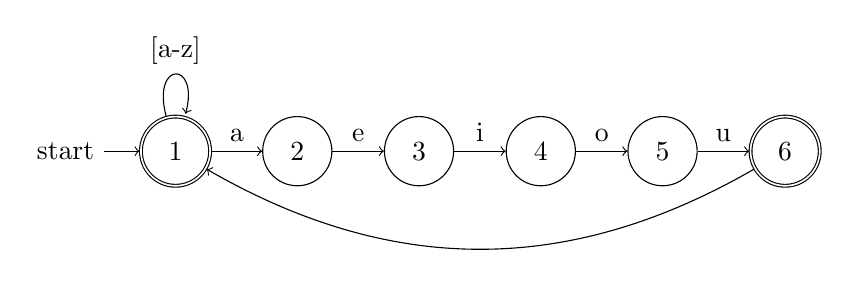
\begin{tikzpicture}
	\node[state, initial, accepting] (q1) {1};
	\node[state, right of=q1, right=0.1cm] (q2) {2};
	\node[state, right of=q2, right=0.1cm] (q3) {3};
	\node[state, right of=q3, right=0.1cm] (q4) {4};
	\node[state, right of=q4, right=0.1cm] (q5) {5};
	\node[state, right of=q5, right=0.1cm, accepting] (q6) {6};

	\draw [->]
		(q1) edge[above] node{a} (q2)
		(q2) edge[above] node{e} (q3)
		(q3) edge[above] node{i} (q4)
		(q4) edge[above] node{o} (q5)
		(q5) edge[above] node{u} (q6)

		(q1) edge[loop above] node{[a-z]} (q1)

		(q6) edge[bend left] node{} (q1)
		;
\end{tikzpicture}
\caption{All strings of lowercase letters that contain the five vowels in order.}
\label{fig:a}
\end{figure}

\begin{figure}[ht]
\centering
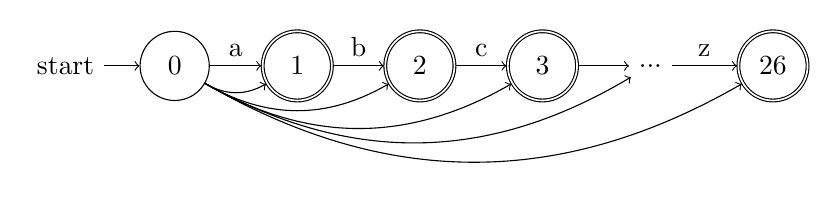
\begin{tikzpicture}
	\node[state, initial] (q1) {0};
	\node[state, right of=q1, right=0.1cm, accepting] (q2) {1};
	\node[state, right of=q2, right=0.1cm, accepting] (q3) {2};
	\node[state, right of=q3, right=0.1cm, accepting] (q4) {3};
	\node[right of=q4, right=0.1cm] (q5) {...};
	\node[state, right of=q5, right=0.1cm, accepting] (q6) {26};

	\draw [->]
		(q1) edge[above] node{a} (q2)
		(q2) edge[above] node{b} (q3)
		(q3) edge[above] node{c} (q4)
		(q4) edge[above] node{} (q5)
		(q5) edge[above] node{z} (q6)

		(q1) edge[bend right] node{} (q2)
		(q1) edge[bend right] node{} (q3)
		(q1) edge[bend right] node{} (q4)
		(q1) edge[bend right] node{} (q5)
		(q1) edge[bend right] node{} (q6)
		;
\end{tikzpicture}
\caption{All strings of lowercase letters in which the letters are in ascending lexicographic order.}
\label{fig:b}
\end{figure}

\begin{figure}[ht]
\centering
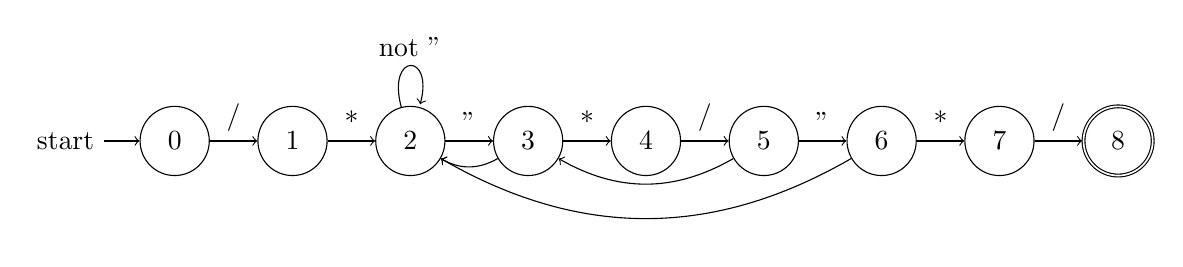
\begin{tikzpicture}
	\node[state, initial] (q1) {0};
	\node[state, right of=q1, right=0.05cm] (q2) {1};
	\node[state, right of=q2, right=0.05cm] (q3) {2};
	\node[state, right of=q3, right=0.05cm] (q4) {3};
	\node[state, right of=q4, right=0.05cm] (q5) {4};
	\node[state, right of=q5, right=0.05cm] (q6) {5};
	\node[state, right of=q6, right=0.05cm] (q7) {6};
	\node[state, right of=q7, right=0.05cm] (q8) {7};
	\node[state, right of=q8, right=0.05cm, accepting] (q9) {8};

	\draw [->]
		(q1) edge[above] node{/} (q2)
		(q2) edge[above] node{*} (q3)
		(q3) edge[above] node{"} (q4)
		(q4) edge[above] node{*} (q5)
		(q5) edge[above] node{/} (q6)
		(q6) edge[above] node{"} (q7)
		(q7) edge[above] node{*} (q8)
		(q8) edge[above] node{/} (q9)

		(q3) edge[loop above] node{not "} (q3)

		(q4) edge[bend left] node{} (q3)
		(q7) edge[bend left] node{} (q3)
		(q6) edge[bend left] node{} (q4)
		;
\end{tikzpicture}
\caption{Comments, consisting of a string surrounded by /* and */, without an intervening */, unless it is inside double-quotes (").}
\label{fig:c}
\end{figure}

\begin{figure}[ht]
\centering
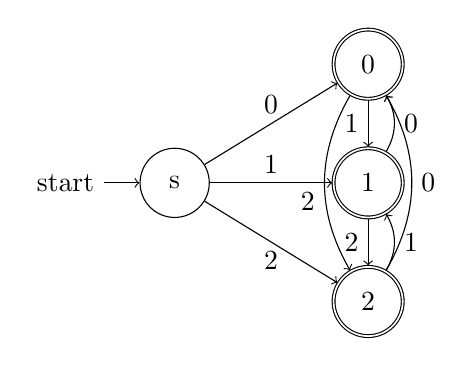
\begin{tikzpicture}
	\node[state, initial] (q1) {s};
	\node[state, right of=q1, right=1cm, accepting] (q3) {1};
	\node[state, above of=q3, above=0.05cm, accepting] (q2) {0};
	\node[state, below of=q3, below=0.05cm, accepting] (q4) {2};

	\draw [->]
		(q1) edge[above] node{0} (q2)
		(q1) edge[above] node{1} (q3)
		(q1) edge[below] node{2} (q4)
		(q2) edge[left] node{1} (q3)
		(q3) edge[left] node{2} (q4)

		(q2) edge[bend right, below left] node{2} (q4)
		(q4) edge[bend right, right] node{0} (q2)
		(q4) edge[bend right, right] node{1} (q3)
		(q3) edge[bend right, right] node{0} (q2)
		;
\end{tikzpicture}
\caption{All strings of digits with no repeated digits. Hint: Try this problem first with a few digits, such as {0, 1, 2}.}
\label{fig:d}
\end{figure}

\begin{figure}[ht]
\centering
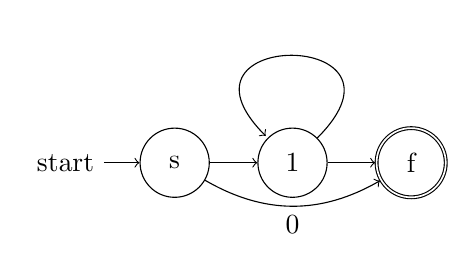
\begin{tikzpicture}
	\node[state, initial] (q1) {s};
	\node[state, right of=q1, right=0.05cm] (q2) {1};
	\node[state, right of=q2, right=0.05cm, accepting] (q3) {f};

	\draw [->]
		(q1) edge[] node{} (q2)
		(q2) edge[] node{} (q3)

		(q2) edge[loop] node{} (q2)

		(q1) edge[bend right, below] node{0} (q3)
		;
\end{tikzpicture}
\caption{All strings of digits with at most one repeated digit.}
\label{fig:e}
\end{figure}

\begin{figure}[ht]
\centering
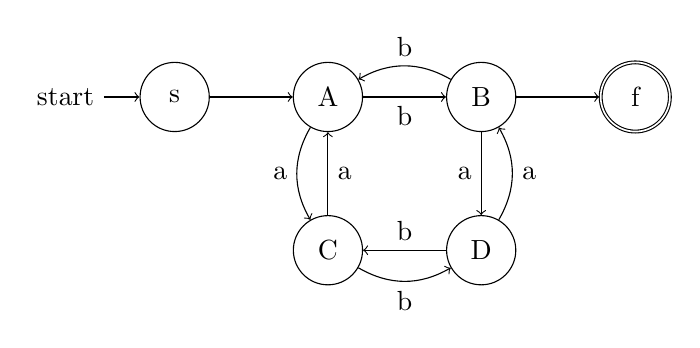
\begin{tikzpicture}
	\node[state, initial] (q1) {s};
	\node[state, right of=q1, right=0.5cm] (q2) {A};
	\node[state, right of=q2, right=0.5cm] (q3) {B};
	\node[state, right of=q3, right=0.5cm, accepting] (q4) {f};
	\node[state, below of=q2, below=0.5cm] (q5) {C};
	\node[state, below of=q3, below=0.5cm] (q6) {D};

	\draw [->]
		(q1) edge[] node{} (q2)
		(q2) edge[below] node{b} (q3)
		(q3) edge[left] node{a} (q6)
		(q6) edge[above] node{b} (q5)
		(q5) edge[right] node{a} (q2)
		(q3) edge[] node{} (q4)

		(q3) edge[bend right, above] node{b} (q2)
		(q2) edge[bend right, left] node{a} (q5)
		(q5) edge[bend right, below] node{b} (q6)
		(q6) edge[bend right, right] node{a} (q3)
		;
\end{tikzpicture}
\caption{All strings of digits with at most one repeated digit.}
\label{fig:f}
\end{figure}

\begin{figure}[ht]
\centering
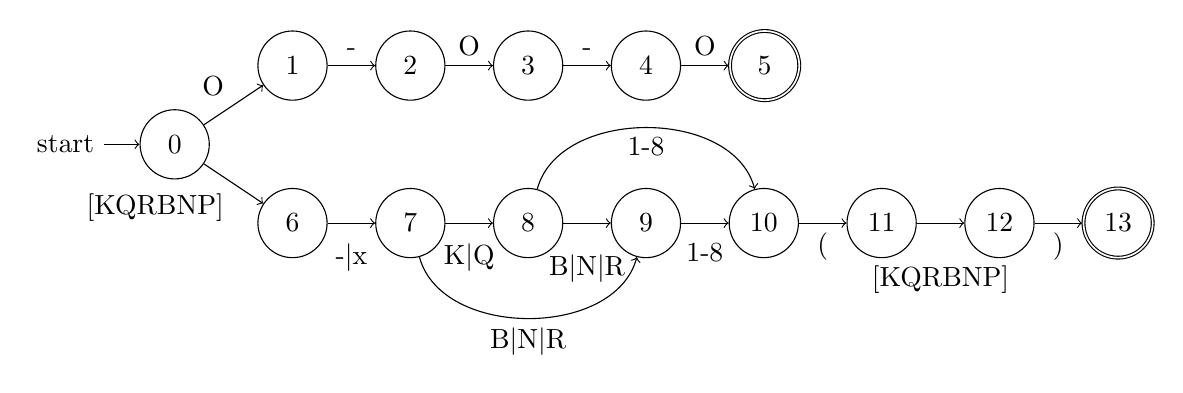
\begin{tikzpicture}[bend angle=75]
	\node[state, initial] (q1) {0};
		\node[state, above of=q1, right of=q1, right=0.05cm] (q2) {1};
		\node[state, right of=q2, right=0.05cm] (q3) {2};
		\node[state, right of=q3, right=0.05cm] (q4) {3};
		\node[state, right of=q4, right=0.05cm] (q5) {4};
		\node[state, right of=q5, right=0.05cm, accepting] (q6) {5};
	\node[state, below of=q1, right of=q1, right=0.05cm] (q7) {6};
	\node[state, right of=q7, right=0.05cm] (q8) {7};
	\node[state, right of=q8, right=0.05cm] (q9) {8};
	\node[state, right of=q9, right=0.05cm] (q10) {9};
	\node[state, right of=q10, right=0.05cm] (q11) {10};
	\node[state, right of=q11, right=0.05cm] (q12) {11};
	\node[state, right of=q12, right=0.05cm] (q13) {12};
	\node[state, right of=q13, right=0.05cm, accepting] (q14) {13};

	\draw [->]
		(q1) edge[above left] node{O} (q2)
		(q2) edge[above] node{-} (q3)
		(q3) edge[above] node{O} (q4)
		(q4) edge[above] node{-} (q5)
		(q5) edge[above] node{O} (q6)

		(q1) edge[below left] node{[KQRBNP]} (q7)
		(q7) edge[below] node[yshift=-4]{-$\vert$x} (q8)
		(q8) edge[below] node[yshift=-4]{K$\vert$Q} (q9)
		(q9) edge[below] node[yshift=-8]{B$\vert$N$\vert$R} (q10)
		(q10) edge[below] node[yshift=-4]{1-8} (q11)
		(q11) edge[below] node{(} (q12)
		(q12) edge[below] node[yshift=-12]{[KQRBNP]} (q13)
		(q13) edge[below] node{)} (q14)

		(q8) edge[bend right, below] node{B$\vert$N$\vert$R} (q10)
		(q9) edge[bend left, below] node{1-8} (q11)
		;
\end{tikzpicture}
\caption{The set of Chess moves, in the informal notation, such as p-k4 or kbpxqn.}
\label{fig:g}
\end{figure}

\begin{figure}[ht]
\centering
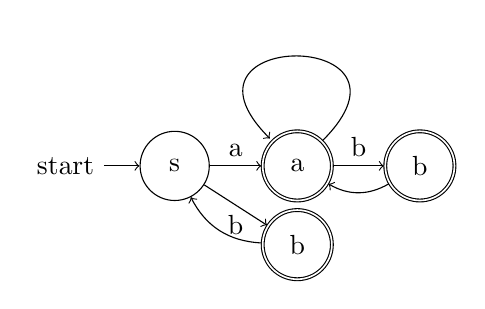
\begin{tikzpicture}
	\node[state, initial] (q1) {s};
	\node[state, right of=q1, right=0.1cm, accepting] (q2) {a};
	\node[state, right of=q2, right=0.1cm, accepting] (q3) {b};
	\node[state, below of=q1, right of=q1, below=0.1cm, right=0.1cm, accepting] (q4) {b};

	\draw [->]
		(q1) edge[above] node{a} (q2)
		(q2) edge[above] node{b} (q3)
		(q1) edge[below] node{b} (q4)

		(q2) edge[loop] node{} (q2)

		(q3) edge[bend left] node{} (q2)
		(q4) edge[bend left] node{} (q1)
		;
\end{tikzpicture}
\caption{All strings of a's and b's that do not contain the substring abb.}
\label{fig:h}
\end{figure}

\begin{figure}[ht]
\centering
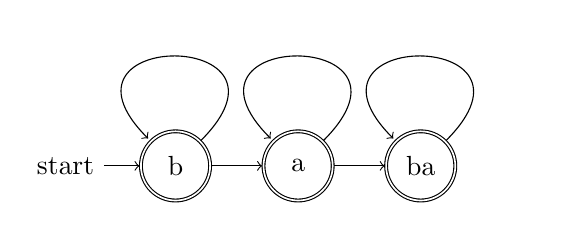
\begin{tikzpicture}
	\node[state, initial, accepting] (q1) {b};
	\node[state, right of=q1, right=0.1cm, accepting] (q2) {a};
	\node[state, right of=q2, right=0.1cm, accepting] (q3) {ba};

	\draw [->]
		(q1) edge[] node{} (q2)
		(q2) edge[] node{} (q3)

		(q1) edge[loop] node{} (q1)
		(q2) edge[loop] node{} (q2)
		(q3) edge[loop] node{} (q3)
		;
\end{tikzpicture}
\caption{All strings of a's and b's that do not contain the subsequence abb.}
\label{fig:i}
\end{figure}

\end{document}
